\documentclass[10pt]{article}
\usepackage[margin=0.7in]{geometry}
\usepackage{amsmath,booktabs,graphicx,microtype,hyperref,float}
\hypersetup{colorlinks=true,urlcolor=blue,citecolor=blue}
\graphicspath{{figures/}}
\setlength{\parskip}{3pt}
\widowpenalty=10000
\clubpenalty=10000
\title{Assignment 2: Federated Learning and Membership Inference}
\author{Team 08 \\ Assignment lead: Chetan Kodand Reddy Madadi \\ Team members: Bharat Govil, Naveen Jarpla, Vishnu Fnu}
\date{Fall 2026}
\begin{document}
\begin{center}
{\Large\bfseries Assignment 2: Federated Learning and Membership Inference\par}
\vspace{4pt}
\textbf{Team 08} \hfill Fall 2026\\
Assignment lead: Chetan Kodand Reddy Madadi\\
Team members: Bharat Govil, Naveen Jarpla, Vishnu Fnu
\end{center}
\begin{abstract}
\textbf{The assignment asks us to implement FedAvg, study how its settings affect
training, test first-round membership inference, and assess whether FL is
practical for our healthcare startup.} We use 9,000 synthetic readmission
encounters, reusing Assignment 1's synthetic data generation pipeline. We compare
28 configurations over three seeds and apply LOSS to every client and global model. \textbf{72 loss-stable endpoints, 9 validation early stops and 3 capped runs.}
The attacks show weak membership discrimination. We distinguish training-loss
stability from selection of a model that generalizes, and discuss what these
results mean for a healthcare startup.
\end{abstract}

\section{Task A: Data, FedAvg, and Experimental Design}
\textbf{Task A asks us to implement FedAvg, vary its settings, train until convergence,
and report test performance after each round.}
Our use case is predicting 30-day readmission at discharge across hospitals.
\textbf{We reused the synthetic data generation pipeline from Assignment 1},
including its cleaning and mixed TabDDPM approach \cite{tabddpm}, based on the
public UCI Diabetes 130-US Hospitals dataset (CC BY 4.0) \cite{uci}.
We use a frozen dataset of 9,000 encounters; 11.22\% have the positive label.
The CSV, schema, integrity audits and hashes accompany the code.
\textbf{Synthetic labels are not verified clinical outcomes, and synthetic data
alone provide no formal privacy guarantee.}

A shared preprocessor, fitted only on public generator seed records, applies
median imputation, numerical standardization and fixed-schema one-hot encoding.
All clients therefore use the same feature coordinates. Synthetic test records
fit no transformation; identifiers and the raw outcome field are excluded.

For seeds 684/685/686, a stratified 50/50 split gives 4,500 training and 4,500
test records. Reserving 900 stratified validation records within the training
half leaves 3,600 for SGD. A fixed shuffle divides them equally and IID among
$K\in\{1,10,20,50\}$ clients (3,600/360/180/72 records each). Splits stay fixed
across settings, with natural finite-sample class variation.

\textbf{Centrally accessible synthetic validation data are an assumption of this
simulation.} The simulated server uses the same 900-record validation set for
LR scheduling, checkpoint selection and prediction-threshold calibration.
A real deployment would need an appropriate validation mechanism, such as an
authorized shared validation set or federated evaluation of locally held-out
data. We do not implement that deployment mechanism here.

\textbf{FedAvg implementation.} The MLP has ReLU hidden widths 128/64 and two
logits. All clients participate every round, using unweighted CE and SGD without
momentum, with L2 weight decay 0.01 on all parameters. Partial batches are kept
at the same LR.
\textbf{Clients start from identical global weights; the server averages their updates:}
\[
W_{r+1}=\sum_{i=1}^{K}\frac{n_i}{\sum_j n_j}W_{i,r+1},
\]
which is the arithmetic mean for equal partitions \cite{fedavg}.
$K=1$ matches centralized SGD with the same epoch grouping and shuffle stream.

\textbf{Parameter study.} Baseline batch size is 32, local epochs one, initial LR 0.05. One parameter at a
time varies over batches $\{16,32,64\}$, epochs $\{1,3,5\}$, and initial LRs
$\{0.01,0.05,0.1\}$. Deduplication gives 28 configurations and 84 seeded runs;
interactions are not tested. \textbf{All plots use seed 684; tables and numerical
comparisons use all three seeds.} After every aggregation, global training,
validation and test CE, accuracy, balanced accuracy, AUROC and average precision
are logged, with runtime, optimizer steps and processed examples.

\textbf{When do we stop, and which model do we report?} A shared validation-CE plateau
scheduler halves LR after 11 bad rounds (PyTorch patience 10), with absolute
improvement tolerance 0.001, cooldown five, and floor initial LR/100.
Let $s_r$ be trailing-ten-round mean training CE. From round 50, each window of
20 smoothed values must have range $\leq\max(5\times10^{-4},0.005d)$ and absolute
OLS slope times 19 $\leq\max(10^{-4},0.001d)$, where
$d=\max(\operatorname{median}(s),10^{-12})$. Require five consecutive passing
windows and one LR throughout their 33-round raw-loss support. Absolute floors avoid excessive precision near zero; persistence and a fixed LR
exclude transient plateaus. We also record the original relative-only bounds.

\textbf{A run stops at loss stability, validation patience, or 300 total rounds,
including resumed rounds.} Predictive patience is 150 rounds without
cumulative validation-CE improvement $>10^{-4}$, eligible from round 80.
The lowest raw validation CE checkpoint (earliest tie) is restored
\cite{modelselection}. Its prediction threshold maximizes validation balanced
accuracy (highest threshold breaks ties). \textbf{Test metrics never control training, stopping, checkpoint selection or
thresholds.} \textbf{The restored checkpoint may precede the stable endpoint.} Neither loss
stability nor early stopping proves a stationary or global optimum. The 12 confirmed baseline training caches are reused unchanged.

\begin{table}[ht]\centering\scriptsize
\caption{Baseline selected-checkpoint results: mean $\pm$ sample SD over three
seeds. Stop rounds are ranges. BA and recall use validation-selected thresholds;
AUROC and CE are threshold-independent. Complete per-round metrics are in CSVs.}
\begin{tabular}{rrlllll}\toprule
$K$ & Stop rounds & Train CE & Test CE & Test AUROC & Test BA & Recall \\
\midrule
1 & 144--197 & 0.2969 $\pm$ 0.0125 & 0.3228 $\pm$ 0.0047 & 0.7066 $\pm$ 0.0180 & 0.6378 $\pm$ 0.0228 & 0.5650 $\pm$ 0.1299 \\
10 & 174--189 & 0.3230 $\pm$ 0.0032 & 0.3314 $\pm$ 0.0023 & 0.6721 $\pm$ 0.0111 & 0.6103 $\pm$ 0.0154 & 0.5947 $\pm$ 0.2341 \\
20 & 184--224 & 0.3257 $\pm$ 0.0019 & 0.3327 $\pm$ 0.0016 & 0.6676 $\pm$ 0.0091 & 0.6135 $\pm$ 0.0048 & 0.6297 $\pm$ 0.0616 \\
50 & 203--234 & 0.3324 $\pm$ 0.0013 & 0.3365 $\pm$ 0.0010 & 0.6568 $\pm$ 0.0039 & 0.6059 $\pm$ 0.0048 & 0.6290 $\pm$ 0.0989 \\
\bottomrule\end{tabular}\end{table}
\begin{figure}[ht]\centering
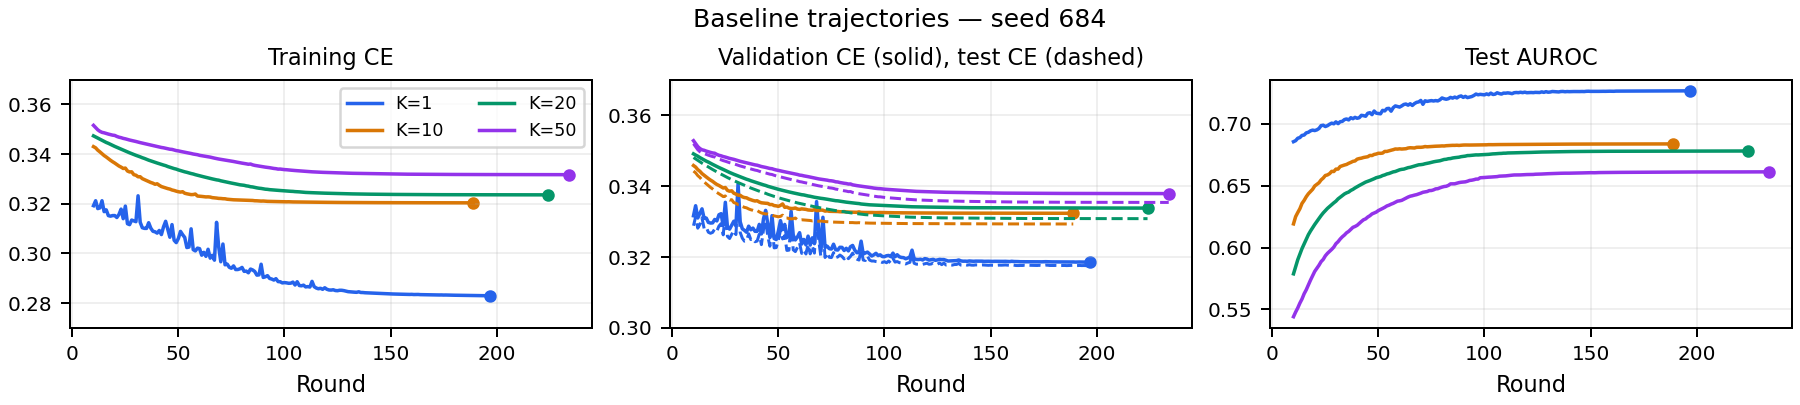
\includegraphics[width=.96\linewidth]{training.png}
\caption{Baseline trajectories for \textbf{seed 684 only}. Colors distinguish
client counts; dots mark validation-selected checkpoints. Rounds 10 onward and restricted CE
axes resolve the plateau; complete histories are in CSV. No extrapolation after stopping.}
\end{figure}

\begin{samepage}
\textbf{Did every run converge?} \textbf{72 of 84 runs reached loss stability; nine stopped on validation patience and three reached the cap.} The stable runs stopped at rounds 144--272, and all also passed the original relative-only loss bounds. Every K=10/20/50 run was stable. All nine early stops and three caps were K=1 variants. The capped settings were B=16/LR=0.05 (seeds 684/685) and B=32/LR=0.1 (seed 684), with E=1. Their last-window fitted CE decrease was 0.000340--0.000527, above their trend limits of 0.000273--0.000290. \textbf{These three runs were still improving slowly, so we retain their unconverged labels.} Early stopping does not establish optimization convergence.
\textbf{Loss stability does not establish good generalization.}\par
\end{samepage}

\begin{table}[ht]\centering\small
\caption{Paired-seed mean changes in selected training CE / test AUROC from the
lowest to highest parameter, with other parameters at baseline. Stop and
selected rounds differ across runs; negative CE indicates better fitting.}
\begin{tabular}{rrrr}\toprule
$K$ & Batch: 16 to 64 & Epochs: 1 to 5 & Initial LR: 0.01 to 0.1 \\
\midrule
1 & +0.0184 / -0.0174 & -0.0272 / +0.0122 & -0.0256 / +0.0293 \\
10 & +0.0074 / -0.0129 & -0.0310 / +0.0356 & -0.0179 / +0.0321 \\
20 & +0.0095 / -0.0158 & -0.0227 / +0.0322 & -0.0220 / +0.0682 \\
50 & +0.0119 / -0.0249 & -0.0148 / +0.0239 & -0.0220 / +0.0870 \\
\bottomrule\end{tabular}\end{table}
\textbf{How do FedAvg settings affect training?} \textbf{More clients meant shorter local update paths and slower learning in the baseline.} Increasing K from 1 to 50 raised mean stop rounds from 167 to 219 and endpoint training CE from 0.2928 to 0.3324; selected test AUROC fell from 0.7066 to 0.6568. Each client takes 113 versus three steps per baseline round. Short local paths change the optimization trajectory.

\textbf{Larger batches reduced computation but weakened fitting and discrimination.} At K=50, increasing B from 16 to 64 reduced mean total steps from 51.6k to 20.5k and recorded time from 76 to 51 s. Selected training CE rose from 0.3271 to 0.3390, while test AUROC fell from 0.6654 to 0.6405.

\textbf{More local epochs saved communication rounds, at a substantial local-computation cost.} At K=50, E=1/3/5 used 219.0/188.7/184.3 mean rounds, 32.9/84.9/138.2k steps, and 0.79/2.04/3.32 million processed examples. Time increased from 61 to 162 s, while AUROC improved from 0.6568 to 0.6807.

\textbf{A small initial learning rate could produce stable but underfit models.} At K=50, LR 0.01 versus 0.1 gave mean selected training CE 0.3471 versus 0.3251 and test AUROC 0.5822 versus 0.6691, despite similar mean stop rounds (207/208). More local work or LR did not guarantee K=1 convergence.
Times include serial clients, evaluation and intermediate checkpoint I/O;
final selection/write and attack reconstruction are excluded. Different CPUs
and execution phases limit timing comparisons; network latency is not simulated.

\textbf{Does better training loss mean better readmission prediction?} \textbf{Regularization and validation selection substantially reduced severe overfitting.} The original fixed-300-round K=1 baseline had mean train/test CE 0.0003/1.2753; the selected model now has 0.2969/0.3228. Across the full grid, selected test CE is 0.3139--0.3495; the largest validation-minus-training and test-minus-training gaps are 0.0788 and 0.0806. Some K=1 overfitting remains.

\textbf{High accuracy alone would hide a clinically important failure.} At the default threshold, 75/84 selected models predict only negatives. Their 88.78\% accuracy simply matches the negative-class prevalence: BA is 0.5 and readmission sensitivity is zero. Validation-selected thresholds produce both classes in all 84 models. Baseline mean BA is 0.6059--0.6378, with recall 56.5--63.0\%. This improves sensitivity at the cost of specificity; it does not improve AUROC or establish clinical usefulness.
Regularization, scheduling, training size and selection changed together; the
historical comparison cannot isolate one cause. \textbf{Validation reused during
protocol development may give optimistic estimates.}

\section{Task B: First-Round LOSS Attacks}
\textbf{Task B asks us to run LOSS after the first round on the global model and
every client model, using the entire dataset.}
The honest-but-curious server follows FedAvg while inspecting individual
returned weights and the aggregated model. For each labelled candidate $(x,y)$,
the score is $-\ell(f(x),y)$: larger scores suggest membership \cite{loss}.
Only round one is attacked, before any validation-driven scheduling decision.
\textbf{Global members are the 3,600 optimization records; global nonmembers are
the 900 validation and 4,500 test records.} A local model's members are its own
optimization partition. \textbf{Local nonmembers are every record outside that
partition}, including other clients' optimization records, validation and test.
Local member/nonmember counts are $3,600/K$ and $9,000-3,600/K$.
Every model scores all 9,000 records.

We report ROC AUC and the highest empirical TPR with FPR at most 1\%, 5\%, or
10\%, preserving tied-score groups rather than interpolating observations.
\textbf{Oracle-threshold balanced accuracy} is
$\max_t[\mathrm{TPR}(t)+1-\mathrm{FPR}(t)]/2$.
\textbf{Membership labels select this threshold retrospectively.} This descriptive quantity is not independently
calibrated attack performance and differs from the classifier's validation
threshold. Every client's results are retained. We average clients within each seed, then
report mean and sample SD over three seeds; clients are not independent replicates.
The audit verifies all 1,785 first-round models, scores and aggregation.

\begin{table}[ht]\centering\scriptsize
\caption{Baseline first-round attacks. Local rows average clients within each
seed; entries are seed mean $\pm$ sample SD. BA is oracle-threshold balanced accuracy.}
\begin{tabular}{rlccccc}\toprule
$K$ & Model & Oracle BA & AUC & TPR@1\% & TPR@5\% & TPR@10\% \\
\midrule
1 & Global & 0.5079 $\pm$ 0.0032 & 0.5023 $\pm$ 0.0067 & 0.0103 $\pm$ 0.0022 & 0.0477 $\pm$ 0.0010 & 0.0939 $\pm$ 0.0019 \\
1 & Local & 0.5079 $\pm$ 0.0032 & 0.5023 $\pm$ 0.0067 & 0.0103 $\pm$ 0.0022 & 0.0477 $\pm$ 0.0010 & 0.0939 $\pm$ 0.0019 \\
10 & Global & 0.5062 $\pm$ 0.0026 & 0.4985 $\pm$ 0.0057 & 0.0072 $\pm$ 0.0024 & 0.0465 $\pm$ 0.0020 & 0.0961 $\pm$ 0.0050 \\
10 & Local & 0.5194 $\pm$ 0.0013 & 0.5045 $\pm$ 0.0037 & 0.0099 $\pm$ 0.0012 & 0.0509 $\pm$ 0.0024 & 0.1015 $\pm$ 0.0059 \\
20 & Global & 0.5062 $\pm$ 0.0032 & 0.4978 $\pm$ 0.0062 & 0.0085 $\pm$ 0.0022 & 0.0483 $\pm$ 0.0014 & 0.0963 $\pm$ 0.0036 \\
20 & Local & 0.5274 $\pm$ 0.0017 & 0.5076 $\pm$ 0.0042 & 0.0094 $\pm$ 0.0011 & 0.0517 $\pm$ 0.0003 & 0.1050 $\pm$ 0.0017 \\
50 & Global & 0.5056 $\pm$ 0.0035 & 0.4970 $\pm$ 0.0054 & 0.0081 $\pm$ 0.0025 & 0.0474 $\pm$ 0.0050 & 0.0952 $\pm$ 0.0036 \\
50 & Local & 0.5413 $\pm$ 0.0023 & 0.5126 $\pm$ 0.0031 & 0.0104 $\pm$ 0.0012 & 0.0565 $\pm$ 0.0026 & 0.1080 $\pm$ 0.0026 \\
\bottomrule\end{tabular}\end{table}

\textbf{Are local attacks stronger, and how do settings affect them?} \textbf{Local LOSS attacks were slightly stronger, but both local and global attacks remained weak.} Baseline global AUROC is 0.4970--0.5023; local AUROC is 0.5023--0.5126. At K=50, the local-minus-global difference is 0.0156.

\textbf{More local work increased the small membership signal.} At K=50, E=1 to 5 raised local AUROC from 0.5126 to 0.5309 and TPR at 1\% FPR from 1.04\% to 1.26\%. B=16 to 64 lowered local AUROC from 0.5180 to 0.5105; initial LR 0.01 to 0.1 raised it from 0.5012 to 0.5189. Global configuration means stayed within 0.4959--0.5062.
\textbf{Our explanation is that aggregation dilutes individual influence, while
small local partitions and more local steps encourage record-specific fitting.}
This is a hypothesis, not a causal finding. Local and global nonmembers have different mixtures, so their
AUC difference cannot isolate aggregation. Oracle BA increases can also reflect
retrospective threshold selection with fewer members. \textbf{Near-chance first-round LOSS does not establish privacy against stronger
attacks}, later-round leakage, or inference about real generator seed patients.

\textbf{Which step needs protection? Sending individual client weights to the
curious server exposes the models used by the local attacks.}
Transport encryption alone does not hide those weights from the receiving
server. \textbf{Secure aggregation hides individual updates by revealing only their
aggregate}, subject to an
appropriate aggregation cohort and dropout/collusion assumptions
\cite{secureagg}; a one-client cohort provides no such protection.
\textbf{The aggregate model can still leak membership; differential privacy
addresses that residual risk.} A formal guarantee requires clipping, calibrated
noise and privacy accounting; noise
must protect updates before the curious server can inspect them, or be applied
inside a trusted aggregation boundary. \textbf{Neither defense is evaluated here} \cite{dp}.

\section{Task C: Practicality and Future of FL}
\paragraph{Why is FL still mostly used in research?}
\textbf{I think the main difficulty is making the extra effort worthwhile.}
Keeping records local is useful, but hospitals still need to agree on features,
coordinate training and deal with different patient populations. Our simple IID
experiment already showed that changing client settings changes training behavior;
a real deployment would add more variation and operational work \cite{survey}.
FL also needs privacy protections beyond keeping raw records local.
Gboard and other Google systems show that production use exists
\cite{gboard,parfait}, but their success does not mean the same setup will suit
our startup. Larger generative models would add communication and resource costs.

\paragraph{What could drive wider adoption?}
\textbf{I would expect adoption to grow when pooling valuable data is difficult
and partners can show a clear benefit from working together.} For hospitals,
that benefit would need to justify the cost of agreeing on a schema, maintaining
the system and evaluating it. Easier tools, convincing privacy guarantees and
examples with measured gains would help. More FL papers alone would not answer
those practical questions.

\paragraph{Would our startup use FL?}
\textbf{I would start with a small cross-hospital pilot, not deploy this model.}
FL is appealing if partners want to collaborate without pooling records.
However, our synthetic results are only an initial check: baseline recall of
56--63\% still misses many positive cases, and changing the threshold creates
false positives. I would want committed partners, agreed features, an appropriate
validation mechanism and privacy protections before proceeding. Our centrally
accessible synthetic validation set is a simulation assumption. We have not
shown that the model works on real, heterogeneous hospital data or that it helps
clinical decisions.

\paragraph{Is there a better alternative?}
\textbf{If pooling is permitted and practical, I would try controlled centralized
training first.} It is simpler to train, debug and compare, although access
controls and privacy protections still matter. If pooling is impossible, local
models avoid shared updates but give up cross-hospital learning. Trusted execution
environments are another option, with hardware and attestation assumptions
\cite{survey,parfait}. I would choose based on the partners' actual constraints,
rather than assume FL is always the better privacy solution.

\textbf{Reproducibility and limits.}
Code, frozen data/partitions, hashes, all 16,088 round records and 1,785 attack
rows accompany the submission; bulky artifacts remain under \texttt{/work}.
Audits and 46 tests verify model/metric consistency, stopping, aggregation,
membership and resume. \textbf{Three seeds, reused validation and synthetic IID
data limit generalization.} Neither defenses nor hospital heterogeneity are
tested; the attack assessment covers first-round LOSS only.

\clearpage
\begin{thebibliography}{10}
\bibitem{uci} J. Clore, K. Cios, J. DeShazo, and B. Strack.
Diabetes 130-US Hospitals for Years 1999--2008. UCI, 2014.
\url{https://doi.org/10.24432/C5230J}.
\bibitem{tabddpm} A. Kotelnikov et al. TabDDPM: Modelling Tabular Data with Diffusion Models.
ICML, 2023. \url{https://arxiv.org/abs/2209.15421}.
\bibitem{fedavg} H. B. McMahan et al. Communication-Efficient Learning of Deep Networks
from Decentralized Data. AISTATS, 2017. \url{https://arxiv.org/abs/1602.05629}.
\bibitem{secureagg} K. Bonawitz et al. Practical Secure Aggregation for Privacy-Preserving
Machine Learning. CCS, 2017. \url{https://eprint.iacr.org/2017/281}.
\bibitem{survey} P. Kairouz et al. Advances and Open Problems in Federated Learning.
Foundations and Trends in Machine Learning, 2021. \url{https://arxiv.org/abs/1912.04977}.
\bibitem{gboard} Google Research. Improving Gboard language models via private federated
analytics. April 19, 2024.
\url{https://research.google/blog/improving-gboard-language-models-via-private-federated-analytics/}.
\bibitem{parfait} Google Research. Parfait: Enabling private AI with research tools.
January 22, 2025. \url{https://research.google/blog/parfait-enabling-private-ai-with-research-tools/}.
\bibitem{modelselection} Scikit-learn developers. Cross-validation: evaluating estimator performance;
MLPClassifier (validation-based early stopping). User Guide and API reference, accessed October 2026.
\url{https://scikit-learn.org/stable/modules/cross_validation.html}.
\url{https://scikit-learn.org/stable/modules/generated/sklearn.neural_network.MLPClassifier.html}.
\bibitem{loss} S. Yeom et al. Privacy Risk in Machine Learning:
Analyzing the Connection to Overfitting. IEEE CSF, 2018.
\url{https://arxiv.org/abs/1709.01604}.
\bibitem{dp} M. Abadi et al. Deep Learning with Differential Privacy.
CCS, 2016. \url{https://arxiv.org/abs/1607.00133}.
\end{thebibliography}
\end{document}
